\begin{figure}
  \centering
  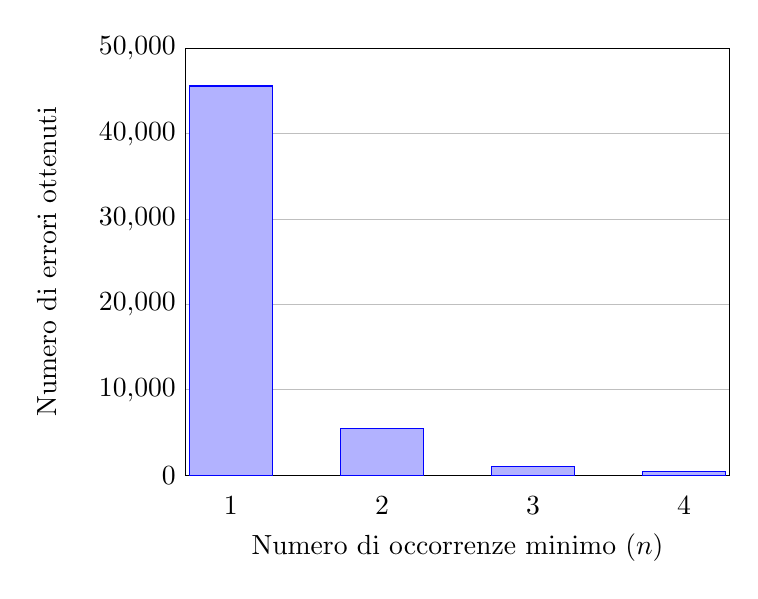
\begin{tikzpicture}
  \begin{axis}[
  width  = \textwidth * 0.7,
  height = 7cm,
  major x tick style = transparent,
  ybar=0.1pt,
  bar width=30pt,
  ymajorgrids = true,
  ylabel style={yshift=2ex},
  xlabel=Numero di occorrenze minimo ($n$),
  ylabel=Numero di errori ottenuti,
  xtick = data,
  scaled y ticks = false,
  ymin=0,ymax=50000,
  ytick style={draw=none},
  %extra y ticks = 100,
  %extra y tick labels={},
  %extra y tick style={grid=major,major grid style={very thick,draw=red}}
  ]
  \addplot table {
    N Numero 
    1 45606
    2 5423
    3 1049
    4 433
  };
  \end{axis}
  \end{tikzpicture}
  \caption{Numero di errori aggregati ottenuti in variazione del numero $n$ di occorrenze minime}
  \label{fig:grafo_aggregazione}
\end{figure}